\section{有限单纯复形}
\label{sec:homol-simplicial-complexes}

要计算洞，先要有能写成有限数据的空间。图是一个候选：它用顶点和边记录直接连接，也可以有环（可参考\BookChapterRef{chap:graph-objects}{卷三第1章“图与连接结构”}）。但本章开头的三角形框与三角形纸片有同一张图，三个顶点两两相邻。图中的环$0\to1\to2\to0$在框上围着一个洞，在纸片上却什么也没围住。

只记录邻接边，就丢掉了“这个环已经被填上”的信息。修补的办法是把“填充”也记下来：除了点和边，还允许记录三个顶点张成的三角形、四个顶点张成的四面体，等等。本节先建立这种有限的组合对象，再把它实现为欧氏空间中的子集，使连续映射与同伦能够作用在它上面。

\subsection{单纯复形的定义}
\label{sec:homol-complex-definition}

一个填充三角形由它的三个顶点确定，一条边由两个端点确定，所以一块“填充”可以简单地记为一个顶点子集。记录要前后一致：填入一个三角形时，它的三条边和三个顶点也必须在记录之中，否则三角形的边缘无处安放。

\begin{definition}[抽象单纯复形]
\label{def:homol-simplicial-complex}
设$V$为有限集。由$V$的非空子集组成的族$\mathcal K$称为以$V$为顶点集的\term{抽象单纯复形}（abstract simplicial complex），若
\begin{itemize}
 \item 对每个$v\in V$，$\{v\}\in\mathcal K$；
 \item 若$\sigma\in\mathcal K$且$\varnothing\neq\tau\subseteq\sigma$，则$\tau\in\mathcal K$。
\end{itemize}
$\mathcal K$中的元素称为\term{单纯形}（simplex）。含$k+1$个顶点的单纯形称为$k$维单纯形，简称$k$-单纯形；单纯形$\sigma$的非空子集称为它的\term{面}（face）。$\mathcal K$中单纯形维数的最大值称为$\mathcal K$的维数。
\end{definition}

第二条要求称为对取面封闭，它正是上面所说的“填入三角形时，边和顶点也要在”。$0$维单纯形是顶点，$1$维单纯形是边，$2$维单纯形是填充三角形，$3$维单纯形是实心四面体。

一维的单纯复形恰好就是一张简单无向图：顶点集是$V$，边集是二元单纯形的全体。单纯复形因而可以看作图向高维的推广。

记$n_k$为$\mathcal K$中$k$维单纯形的个数。若$\mathcal L\subseteq\mathcal K$本身也是单纯复形，就称$\mathcal L$为$\mathcal K$的\term{子复形}（subcomplex）。维数不超过$k$的单纯形组成的子复形称为$\mathcal K$的$k$维\term{骨架}（skeleton），记为$\mathcal K^{(k)}$；一维骨架就是$\mathcal K$的顶点与边组成的图。

\begin{example}[三角形边界与填实三角形]
\label{ex:homol-two-triangles}
取$V=\{0,1,2\}$，令
\begin{align*}
 \mathcal T_1&=\bigl\{\{0\},\{1\},\{2\},\{0,1\},\{1,2\},\{0,2\}\bigr\},\\
 \mathcal T_2&=\mathcal T_1\cup\bigl\{\{0,1,2\}\bigr\}.
\end{align*}
两者都对取面封闭。$\mathcal T_1$是一维复形，单纯形个数为$(n_0,n_1)=(3,3)$，记录三角形的边界；$\mathcal T_2$是二维复形，单纯形个数为$(n_0,n_1,n_2)=(3,3,1)$，记录填实的三角形。

它们的一维骨架相同，都是三个顶点两两相邻的图，$\mathcal T_1$是$\mathcal T_2$的子复形。集合族$\bigl\{\{0\},\{1\},\{2\},\{0,1,2\}\bigr\}$则不是单纯复形，它记录了三角形，却缺少三条边。
\end{example}

图~\ref{fig:homol-triangle-complexes}的前三幅画出了这三个集合族。比较(a)与(b)，例~\ref{ex:homol-two-triangles}说明图中的环未必对应复形中的洞：在$\mathcal T_2$中，环$0\to1\to2\to0$恰好是那个填充三角形的边界。判断一个环是否围住了洞，要看它能否被某些高维单纯形“填掉”，第~\ref{sec:homol-simplicial-homology}节用边界映射把这件事说精确。

\begin{BookInlineFigure}
  \centering
  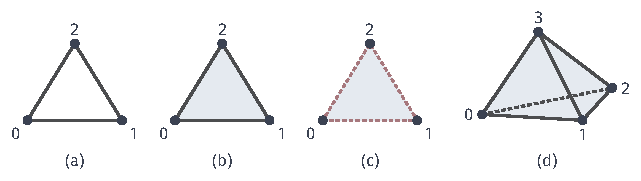
\includegraphics[width=108.532mm]{figures/04-spaces-measures-and-geometry/01-topology-and-metric/tikz/homol-triangle-complexes/figure.pdf}
  \caption{有限单纯复形及一个反例。(a)$\mathcal T_1$：三角形边界。(b)$\mathcal T_2$：填实的三角形，比(a)多一个二维单纯形（浅蓝）。(c)只有填充和顶点、没有三条边的集合族（红色虚线表示缺失的边），不对取面封闭。(d)$\mathcal S$：空心四面体表面，虚线是被遮挡的边，内部没有三维单纯形。}
  \label{fig:homol-triangle-complexes}
\end{BookInlineFigure}

\begin{example}[四面体的表面]
\label{ex:homol-tetrahedron-boundary}
取$V=\{0,1,2,3\}$，令$\mathcal S$由$V$的全部非空真子集组成，即$4$个顶点、$6$条边和$4$个三角形，单纯形个数为$(n_0,n_1,n_2)=(4,6,4)$，不含$3$维单纯形$\{0,1,2,3\}$。它记录空心四面体的表面，见图~\ref{fig:homol-triangle-complexes}(d)，中间围住一个“二维的洞”。再加上$V$本身，就得到实心四面体。
\end{example}

\subsection{几何实现}
\label{sec:homol-geometric-realization}

抽象单纯复形只是集合族，没有点、开集或连续映射。要谈论同伦，必须把它变成一个拓扑空间：每个$k$维单纯形换成一块$k$维的“实心”几何对象，再把公共的面粘在一起。

\paragraph{标准单纯形}
先定下这块几何对象。在$\mathbb R^{k+1}$中，取坐标非负且和为$1$的点，得到
\begin{equation}
 \Delta^k=\Bigl\{\bm t=(t_0,\ldots,t_k)\in\mathbb R^{k+1}:t_i\geq0,\ \sum_{i=0}^kt_i=1\Bigr\},
 \label{eq:homol-standard-simplex}
\end{equation}
称为$k$维\term{标准单纯形}（standard simplex），取$\mathbb R^{k+1}$的子空间拓扑。它是标准基向量$\bm e_0,\ldots,\bm e_k$的凸包，有界且闭，因而紧。

$\Delta^0$是一点，$\Delta^1$是线段，$\Delta^2$是三角形，$\Delta^3$是四面体，图~\ref{fig:homol-standard-simplices}画出了后三者。坐标$t_i$可以读成“$\bm e_i$的权重”：$\Delta^2$中的点$\bm t=(\frac12,\frac14,\frac14)$就是
\[
 \tfrac12\bm e_0+\tfrac14\bm e_1+\tfrac14\bm e_2,
\]
三个顶点的加权平均。把某些坐标取为零，得到的子集仍是由其余基向量张成的低维单纯形，称为$\Delta^k$的面。例如$\Delta^2$中$t_0=0$的点组成连接$\bm e_1,\bm e_2$的边。

\begin{BookInlineFigure}
  \centering
  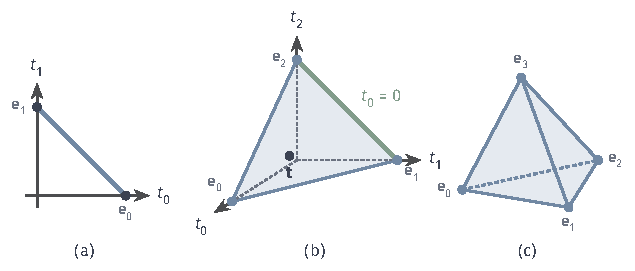
\includegraphics[width=107.453mm]{figures/04-spaces-measures-and-geometry/01-topology-and-metric/tikz/homol-standard-simplices/figure.pdf}
  \caption{标准单纯形。(a)$\Delta^1$是$\mathbb R^2$中连接$\bm e_0,\bm e_1$的线段。(b)$\Delta^2$是$\mathbb R^3$中的三角形，黑点是$\bm t=(\frac12,\frac14,\frac14)$；绿色边是$t_0=0$的面。(c)$\Delta^3$位于$\mathbb R^4$中，此处按四面体形状示意，虚线是被遮挡的边。}
  \label{fig:homol-standard-simplices}
\end{BookInlineFigure}

\paragraph{沿公共面粘合}
下面把单纯形按记录粘起来。设$\mathcal K$的顶点集为$V$。对每个单纯形$\sigma\in\mathcal K$，取一份以$\sigma$的顶点为坐标编号的几何单纯形：
\[
 \Delta^\sigma=\Bigl\{(t_v)_{v\in\sigma}:t_v\geq0,\ \sum_{v\in\sigma}t_v=1\Bigr\}.
\]

把各份放在某个欧氏空间中互不相交的位置，它们的并记为$W$，取子空间拓扑。$W$是有限个紧集之并，因而紧。若$\tau\subseteq\sigma$，则$\Delta^\tau$可以看作$\Delta^\sigma$中$\sigma\setminus\tau$各坐标为零的那个面。

在$W$上规定：$\Delta^\tau$中的点与$\Delta^\sigma$中对应面上坐标相同的点等价，并取由此生成的等价关系$\sim$。商空间$W/{\sim}$（第~\ref{chap:topological-spaces}章）就是把每个面与它在复形中对应的单纯形粘成一份，图~\ref{fig:homol-gluing}(a)(b)画的是两个三角形沿公共边粘合的情形。

\begin{BookInlineFigure}
  \centering
  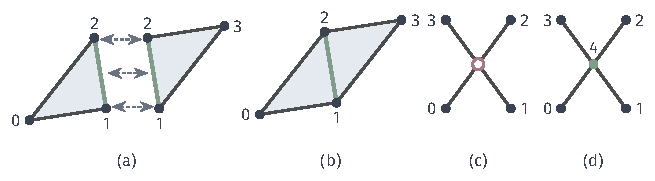
\includegraphics[width=110.973mm]{figures/04-spaces-measures-and-geometry/01-topology-and-metric/tikz/homol-gluing/figure.pdf}
  \caption{粘合与画法。(a)$\{0,1,2\}$与$\{1,2,3\}$的两份几何单纯形，公共边的两份副本为绿色，虚线箭头连接被等同的点。(b)粘合结果。(c)边$\{0,2\}$与$\{1,3\}$在纸上交叉，但红色空心点不是复形中的点。(d)加入新顶点$4$并把两条边各拆成两段之后，四条边才在$4$相遇。}
  \label{fig:homol-gluing}
\end{BookInlineFigure}

这个商空间可以直接放进欧氏空间。把顶点集写成$V=\{v_1,\ldots,v_n\}$，在$\mathbb R^n$中令顶点$v_j$对应标准基向量$\bm e_j$，记
\begin{equation}
 \lvert\mathcal K\rvert=\bigcup_{\sigma\in\mathcal K}\operatorname{conv}\{\bm e_j:v_j\in\sigma\}\subseteq\mathbb R^n,
 \label{eq:homol-realization}
\end{equation}
取子空间拓扑，其中$\operatorname{conv}$表示凸包。

$\lvert\mathcal K\rvert$中的点$\bm x=\sum_jx_j\bm e_j$满足$x_j\geq0$、$\sum_jx_j=1$，这些坐标称为\term{重心坐标}（barycentric coordinates），坐标为正的顶点组成的集合称为它的支撑。重心坐标告诉我们这个点是哪些顶点的加权平均，支撑告诉我们它落在哪一块单纯形的“内部”。

\begin{lemma}[几何单纯形只在公共面上相交]
\label{lem:homol-simplices-intersect}
在式~\eqref{eq:homol-realization}中，点$\bm x$属于$\sigma$对应的凸包，当且仅当它的支撑包含于$\sigma$。因此$\sigma,\tau$对应的两个凸包之交恰为$\sigma\cap\tau$对应的凸包；当$\sigma\cap\tau=\varnothing$时，二者不相交。每个点的支撑本身是$\mathcal K$中的一个单纯形。
\end{lemma}

\begin{proof}
$\sigma$对应的凸包由非负、和为一、且在$\sigma$以外的坐标为零的向量组成，所以$\bm x$属于它当且仅当支撑包含于$\sigma$。

两个凸包都含$\bm x$，当且仅当支撑同时包含于$\sigma$与$\tau$，即包含于$\sigma\cap\tau$，这恰好是$\bm x$属于$\sigma\cap\tau$对应的凸包。

若$\bm x$属于某个$\sigma$对应的凸包，它的支撑是$\sigma$的非空子集，由取面封闭性仍属于$\mathcal K$。
\end{proof}

现在比较商空间$W/{\sim}$与$\lvert\mathcal K\rvert$。把$\Delta^\sigma$中的点$(t_v)_{v\in\sigma}$送到$\sum_{v_j\in\sigma}t_{v_j}\bm e_j$，得到连续满射$\Phi:W\to\lvert\mathcal K\rvert$。

两点被$\Phi$送到同一点，当且仅当它们有相同的非零坐标。记这些坐标所在的顶点集为$\rho$，由引理~\ref{lem:homol-simplices-intersect}它是一个单纯形，两点都是$\Delta^\rho$中同一点在各自单纯形的面上的副本，恰好被$\sim$等同。所以$\Phi$诱导出连续双射
\[
 \bar\Phi:W/{\sim}\to\lvert\mathcal K\rvert.
\]

要说明$\bar\Phi$是同胚，还需要逆映射连续。下面的引理把这一步化成紧性，这也是拓扑中判定同胚最常用的手段。

\begin{lemma}[紧空间到Hausdorff空间的连续双射]
\label{lem:homol-compact-hausdorff}
设$X$紧，$Y$是Hausdorff空间，$f:X\to Y$是连续双射，则$f$是同胚。
\end{lemma}

\begin{proof}
只需证明$f$把闭集映为闭集，这样$f^{-1}$作用下闭集的原像是闭集，$f^{-1}$连续。

设$F\subseteq X$闭。紧空间的闭子集是紧的，紧集的连续像是紧的，所以$f(F)$紧。

还要说明Hausdorff空间中的紧集$C$是闭集。任取$y\notin C$，对每个$c\in C$取$y$的邻域$U_c$与$c$的邻域$V_c$使二者不交。各$V_c$覆盖$C$，由紧性有有限子覆盖；相应有限个$U_c$之交是$y$的邻域，它与$C$不交。所以$C$的补集是开集，$f(F)$是闭集。
\end{proof}

$W$紧，商映射连续，所以$W/{\sim}$紧。$\lvert\mathcal K\rvert$是欧氏空间的子集，是Hausdorff空间。由引理~\ref{lem:homol-compact-hausdorff}，$\bar\Phi$是同胚。我们把$\lvert\mathcal K\rvert$称为$\mathcal K$的\term{几何实现}（geometric realization）。若拓扑空间$X$同胚于某个$\lvert\mathcal K\rvert$，就称$\mathcal K$是$X$的一个\term{三角剖分}（triangulation）。

\paragraph{抽象顶点、坐标与空间}
几何实现涉及三个层次，不能混淆。抽象顶点只是$V$中的名字。坐标表示是选定的嵌入，例如式~\eqref{eq:homol-realization}用标准基向量，也可以用平面上的三个点实现$\mathcal T_2$。空间本身则是同胚意义下确定的对象。

换一种坐标表示，只要每个单纯形实现为相应顶点的凸包，且不同单纯形只在公共面上相交，得到的空间就与$\lvert\mathcal K\rvert$同胚，理由与上面相同。这与线性代数中“向量本身与它的坐标”的区别是同一回事：选坐标是为了计算，选法不影响对象。

\begin{example}[三角形边界是圆周]
\label{ex:homol-triangle-circle}
把$\mathcal T_1$的三个顶点实现为平面上一个三角形的三个顶点，三条边实现为三条边线，得到三角形边线$T\subseteq\mathbb R^2$。取三角形的重心$\bm c$，考虑径向投影
\[
 \bm x\mapsto\frac{\bm x-\bm c}{\lVert\bm x-\bm c\rVert_2},\qquad T\to S^1.
\]
从$\bm c$出发的每条射线恰好与$T$交于一点，所以这是连续双射。$T$紧，$S^1$是Hausdorff空间，由引理~\ref{lem:homol-compact-hausdorff}，它是同胚，所以$\lvert\mathcal T_1\rvert\cong S^1$。

对填实的三角形，沿每条从$\bm c$出发的射线做线性伸缩，把射线上落在三角形内的线段拉成单位长度。三角形写成三个半平面$\langle\bm n_e,\bm x-\bm c\rangle\leq d_e$（$d_e>0$）的交，令
\[
 p(\bm v)=\max_e\frac{\langle\bm n_e,\bm v\rangle}{d_e},
\]
这样$\bm x$在三角形内当且仅当$p(\bm x-\bm c)\leq1$，$p$是连续函数。令$G(\bm c)=\bm 0$，其余点令
\[
 G(\bm x)=p(\bm x-\bm c)\,\frac{\bm x-\bm c}{\lVert\bm x-\bm c\rVert_2}.
\]
$G$是从三角形到$D^2$的连续双射，再由引理~\ref{lem:homol-compact-hausdorff}得$\lvert\mathcal T_2\rvert\cong D^2$。同样的径向投影给出$\lvert\mathcal S\rvert\cong S^2$。
\end{example}

画在纸上的图形却可能误导。取$V=\{0,1,2,3\}$与
\[
 \mathcal K=\bigl\{\{0\},\{1\},\{2\},\{3\},\{0,2\},\{1,3\}\bigr\},
\]
把四个顶点画在正方形的四角，两条边画成两条对角线，纸上的线段在中心交叉，如图~\ref{fig:homol-gluing}(c)所示。

由引理~\ref{lem:homol-simplices-intersect}，$\{0,2\}$与$\{1,3\}$不交，它们的实现在$\mathbb R^4$中也不相交：$\lvert\mathcal K\rvert$是两条互不相交的线段，而不是一个“X”形。画法中的交叉点不是复形中的点。要表示两条边在中间相遇，必须在复形中加入一个新顶点，并把两条边各拆成两段，如图~\ref{fig:homol-gluing}(d)所示。
